% !TeX program = lualatex
% !TeX encoding = utf8
% !TeX spellcheck = uk_UA
% !BIB program = biber
% !TEX indexprogram = upmendex

% chktex-file 1
% chktex-file 3
% chktex-file 12
% chktex-file 24
% chktex-file 25

\documentclass[biblatex]{ConspectBook}

%===============================================================================
%
%							Вихідні дані докумета
%
%===============================================================================

\title{Електрика та магнетизм}
\def\subtitle{Підручник}
\def\authors{С.~М.~Пономаренко}

%=================================== Бібліографія  =============================
%
\addbibresource{d:/Projects/LaTeX/MyPackages/bib/MyBase.bib}
\addbibresource{./bibliography/Articles.bib}

%\addbibresource{Kvant.bib}
%
%===============================================================================

%===============================================================================
%
% !TeX root =./ClassicalElectrodynamics.tex

% chktex-file 1

%========================================================================================================
%
%									      Протоколи
%
%========================================================================================================


% ============ НН ФТІ ==========
\newcommand\IPTNo{13}            % Номер протокола затвердження методичною комісією НН ФТІ
\newcommand\IPTDate{26.10.2026}  % Дата протокола затвердження методичною комісією НН ФТІ

% ============ КПІ =============
\newcommand\KPINo{X}             % Номер протокола надання грифу КПІ
\newcommand\KPIDate{XX.XX.2026}  % Дата протокола надання грифу КПІ

%========================================================================================================
%
%									      Палітурка
%
%========================================================================================================

\newcommand{\CoverPage}{
	\begin{alwayssingle}
		\begin{center}
			\begin{flushright}\bfseries\sffamily
				\MakeUppercase{Міністерство освіти і науки України}\\
				КПІ ім. Ігоря Сікорського\\
			\end{flushright}
			\begin{tcolorbox}[titlepagestyle,
					toprule=0.10cm,
					bottomrule=0.10cm,
					overlay={%
							\node (picture) at ([xshift=4cm]frame.west) {
\includegraphics[width=3.5cm]{logo/logo_IPT}};
						}
				]%
				\begin{flushright}
					\large\bfseries\color{white}Навчально-науковий\\ фізико-технічний інститут
				\end{flushright}
			\end{tcolorbox}
			\vspace*{-2em}
			\begin{Large}\color{themecolordark!90!black}
				\begin{alignat*}{3}
					\vect{\nabla} & \times  &  & \Efield &  & = -\dfrac{1}{c}\dfrac{\partial\Bfield}{\partial t}                         \\
					\vect{\nabla} & \,\cdot &  & \Bfield &  & = 0                                                                        \\
					\vect{\nabla} & \,\cdot &  & \Dfield &  & = 4\pi\rho                                                                 \\
					\vect{\nabla} & \times  &  & \Hfield &  & = \dfrac{4\pi}{c} \vect{j}+\dfrac{1}{c}\dfrac{\partial\Dfield}{\partial t}
				\end{alignat*}
			\end{Large}
			\vspace*{2em}
			\begin{tcolorbox}[
					titlepagestyle,
					toprule=0.15cm,
					bottomrule=0.15cm,
					top=1.3cm,
					bottom=0.7cm,
					overlay={%
							\node[%
								fill=white,
								rounded corners = 15pt,
								draw=themecolorlight,
								line width=0.15cm,
								inner sep=0pt,
								text width=17cm,
								minimum height=2cm,
								align=center,
								%anchor=east,
								font=\sffamily\bfseries\large
							] (title) at (frame.north) {С.~М. Пономаренко
							};
						}
				]
				\centering
				\Huge\sffamily\bfseries\textcolor{white}{\realtitle}\\
				\huge\sffamily\bfseries\textcolor{white}{\subtitle}
			\end{tcolorbox}
			\vfill
			% Адаптовано з MaxwellEqns.tex (слайд "Стаціонарні поля")
\begin{minipage}[t]{0.3\linewidth}\centering
	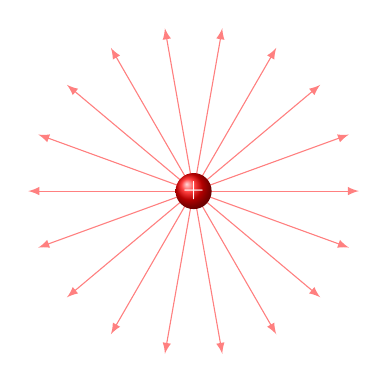
\begin{tikzpicture}[>=latex, scale=1]
		\foreach \i in {20,40,...,360}
			{
				\draw[->, red!50] (0,0)  ++(\i:0.1) -- ++(\i:2);
			}
		\node[circle, inner sep=1pt, ball color=red, text=white] at (0, 0) {$+$};
	\end{tikzpicture}
\end{minipage}
\begin{minipage}[t]{0.3\linewidth}\centering
	\begin{tikzpicture}[>=latex, scale=1]
		\draw [in=-105, out=75, looseness=1.25, line width=0.1cm, gray!50] (-1, -1) coordinate (A)
		to (1, 1.5) coordinate (B);
		\draw[fill=gray!50, ultra thin, rotate around={-10:(B)}] (B) circle(0.05 and 0.015);
		\draw[fill=gray!50, ultra thin, rotate around={-10:(A)}] (A) circle(0.05 and 0.015);
		\draw[thin, blue, rotate around={-15:(-0.25:0)}, arrowpos={0.85}{2pt}{4pt}] (-0.25, 0)
		circle(0.5 and 0.15);
		\draw[thin, blue, rotate around={-15:(-0.25:0)}, arrowpos={0.85}{2pt}{4pt}] (-0.25, 0)
		circle(2 and 0.7);
		\draw[thin, blue, rotate around={-15:(-0.25:0)}, arrowpos={0.85}{2pt}{4pt}] (-0.25, 0)
		circle(1 and 0.3);
		\begin{scope}
			\clip (-1,0) rectangle (1,1);
			\draw [in=-105, out=75, looseness=1.25, line width=0.1cm, gray!50] (A) to (B) ;
		\end{scope}
		\draw [in=-105, out=75, looseness=1.25, gray, arrowpos={0.85}{2pt}{4pt}] (-1, -1)
		coordinate (A) to (1, 1.5) coordinate (B);
	\end{tikzpicture}
\end{minipage}
\begin{minipage}[t]{0.3\linewidth}\centering
\begin{tikzpicture}[rotate=90, scale=1, >=latex, midarrow/.style={%
				postaction={ decorate,
						decoration={ markings, mark=at position .7 with {\arrow{latex}}}}}]
	\begin{scope}[xshift=0.3cm]
		\draw[arrowpos={0.5}{2pt}{4pt}, red] (1.1,0) [partial ellipse=360:0:0.15 and 0.5];
		\draw[arrowpos={0.5}{2pt}{4pt}, red] (1.1,0) [partial ellipse=360:0:0.3 and 1];
		\draw[arrowpos={0.5}{2pt}{4pt}, red] (1.1,0) [partial ellipse=360:0:0.6 and 2] node[pos=0.5,
		below] {$\Efield$};
	\end{scope}
	\foreach \y in {-3,...,3}{
			\draw[blue, midarrow] plot[domain=1:3] (\x, 0.2*\y+0.05*\y*\x^2);
		}
	\node[blue, font=\small] at (3.5, 0) {$\frac{\partial\Bfield}{\partial t}>0$};
\end{tikzpicture}
\end{minipage}


			\vfill
			\begin{tcolorbox}[titlepagestyle,
					toprule=0.10cm,
					bottomrule=0.10cm]
				\begin{center}\color{white}\bfseries\normalsize
					\MakeUppercase{Київ~\the\year} \\
					%					КПІ ім. Ігоря Сікорського \\
					%					\the\year
				\end{center}
			\end{tcolorbox}
		\end{center}
		\clearpage
	\end{alwayssingle}
	\setcounter{page}{1}
}


%========================================================================================================
%
%									      Титульна сторінка
%
%========================================================================================================

\renewcommand\maketitle{
	\begin{alwayssingle}
		\begin{center}
			\MakeUppercase{Міністерство освіти і науки України}

			\bigskip
			\MakeUppercase{Національний технічний університет України}\\
			<<КИЇВСЬКИЙ ПОЛІТЕХНІЧНИЙ ІНСТИТУТ \\ імені ІГОРЯ СІКОРСЬКОГО>>
			\vspace*{100pt}

			{\large С.~М.~Пономаренко
			}
			\vspace*{50pt}

			{\Huge\sffamily\bfseries\realtitle}\\[1em]
			{\huge\sffamily\bfseries\subtitle}

			\vspace*{50pt}
			\begin{center}\itshape
				Затверджено Вченою радою КПІ ім. Ігоря Сікорського як підручник для
				здобувачів ступеня бакалавра за спеціальностями E6 Прикладна фізика та наноматеріали.
			\end{center}
			\vfill
			%                 \textcolor{malina}{Видання друге, виправлене та доповнене}
			%                \textcolor{malina}{Версія від~\today, час компіляції \currenttime.}
			\vfill
			\begin{center}
				\MakeUppercase{Київ} \\
				КПІ ім. Ігоря Сікорського \\
				\the\year
			\end{center}
		\end{center}
		\clearpage
	\end{alwayssingle}
}


%========================================================================================================
%
%									      Друга сторінка
%
%========================================================================================================
\newcommand\makeinfopage{
	\begin{alwayssingle}
		\noindent%
		\begin{minipage}[t]{0.5\textwidth}
			\begin{flushleft}
				УДК  537(075.8)\\
				ББК  22.31я73\\
				П 563
			\end{flushleft}
		\end{minipage}


		\bigskip\noindent%
		\begin{minipage}[t]{0.25\linewidth}
			\begin{flushleft}
				Рецензенти:
			\end{flushleft}
		\end{minipage}\hfill
		\begin{minipage}[t]{0.75\linewidth}
			\href{https://staff.lpnu.ua/profile/Ihor.R.Zachek}{І.~Р.~Зачек}, д.ф.-м.н.,
			професор кафедри загальної фізики Інституту прикладної математики та
			фундаментальних наук Національного університету <<Львівська політехніка>>.
			\\[1ex]
			\href{https://esu.com.ua/article-76544}{О.~Я.~Оліх}, д.ф.-м.н., професор,
			завідувач кафедри загальної фізики, фізичного факультету КНУ імені Тараса
			Шевченка.
		\end{minipage}

		\bigskip\noindent%
		\begin{minipage}[t]{0.25\linewidth}
			\begin{flushleft}
				Відповідальний редактор:
			\end{flushleft}
		\end{minipage}\hfill
		\begin{minipage}[t]{0.75\linewidth}
			\href{https://is.ipt.kpi.ua/is/litvinovatv/}{Т.~В.~Литвинова}, к.т.н.,
			доцент, перший заступник директора НН ФТІ КПІ ім. Ігоря Сікорського.
		\end{minipage}

		\vfill

		\begin{center}\itshape\small
			Гриф надано Вченою радою КПІ ім. Ігоря Сікорського (протокол №~\KPINo~від \KPIDate~р.) за поданням Вченої ради Навчально-наукового Фізико-технічного інституту (протокол №~\IPTNo~від \IPTDate~р.)
		\end{center}
		\vfill
		% 		\begin{center}
		% 			\ifelectronic Електронне мережне навчальне видання \fi
		% 			%\par {Версія від~\href{http://www.istpravda.com.ua/dates}{\today}} \par\else \par  \fi
		% 		\end{center}
		% 		\begin{center}
		% 			\href{https://apd.ipt.kpi.ua/kafedra/stuff/ponomarenko}{\itshape Пономаренко Сергій
		% 			Миколайович}, к.ф.-м.н., доцент
		% 		\end{center}
		% %			\vspace*{1em}%
		% 		\begin{center}\bfseries
		% 			\LARGE\sffamily\realtitle \\
		% 			\Large\sffamily\subtitle
		% 		\end{center}

		% ========================================================
		\noindent
		\phantom{П 563}\hfill%
		\begin{minipage}[t]{0.85\textwidth}\small
			\textbf{Пономаренко С.М.}
		\end{minipage}
		% ========================================================

		\noindent%
		П 563\hfill \begin{minipage}[t]{0.85\textwidth}\small
			\hspace{2em}\realtitle\ [Електронний ресурс] : підруч. для студ. спеціальностей
			E6 <<Прикладна фізика та наноматеріали>> / С.~М. Пономаренко; КПІ ім. Ігоря Сікорського.~--- Електронні
			текстові дані
			(1 файл: 16{,}6~МБ). – Київ: КПІ ім. Ігоря Сікорського, \the\year. ---
			\the\numexpr\getpagerefnumber{LastPages}-1\relax~с.
		\end{minipage}

		%		\noindent%
		%		\begin{flushleft}
		%			\begin{tabular}{lp{0.9\textwidth}}
		%				     & В.~І. Жданов, С.~М. Пономаренко, В.~Б. Долгошей                                                                                                                                                                        \\
		%				Ж 42 & \hspace*{3ex} \realtitle : \subtitle{} [Електронний ресурс] : навчальний посібник / %
		%				В.~І. Жданов, %
		%				С.~М. Пономаренко%,
		%				В.~Б. Долгошей %
		%				--- К.:~КПІ ім. Ігоря Сікорського, \the\year. --~\the\numexpr\getpagerefnumber{LastPage}-1\relax~с. -- Бібліогр.: с.~\pageref{BibPage}\relax. \ifelectronic\relax\else-- 80~прим.\fi
		%			\end{tabular}
		%		\end{flushleft}
		\vfill


		Для студентів фізико-технічного інституту КПІ ім. Ігоря Сікорського, які навчаються за спеціальностями E6~Прикладна фізика та наноматеріали.

		\vfill

		\begin{center}\scriptsize
			Реєстр. № П ХХ/ХХ-ХХХ. Обсяг Х,Х авт. арк.\\
			Національний технічний університет України \\
			«Київський політехнічний інститут імені Ігоря Сікорського»\\
			проспект Берестейський, 37, м. Київ, 03056\\
			\url{https://kpi.ua}\\
			Свідоцтво про внесення до Державного реєстру видавців, виготовлювачів \\
			і розповсюджувачів видавничої продукції ДК № 5354 від 25.05.2017 р.
		\end{center}

		\vfill
		
		\begin{flushright}
			\begin{minipage}[t]{0.6\linewidth}\small
				\textcopyright{} С.~М. Пономаренко, \the\year\,р. \\
				\textcopyright{}  КПІ ім. Ігоря Сікорського (НН ФТІ), \the\year~р.
			\end{minipage}
		\end{flushright}
		\newpage%
	\end{alwayssingle}
}

%%%%%%%%%%%%%%%%%%%%%%%%%%%%%%%%%%%%%%%%%%%%%%%%%%%%%%%%%%%%%%%%%%%%%%%%%%%%
%%                                                                        %%
%%                              Last Page                                 %%
%%                                                                        %%
%%%%%%%%%%%%%%%%%%%%%%%%%%%%%%%%%%%%%%%%%%%%%%%%%%%%%%%%%%%%%%%%%%%%%%%%%%%%
\newcommand{\makelastpage}{%
	\clearpage%
	\thispagestyle{empty}%
	\vspace*{0.4\textheight}
	\begin{center}
		\textbf{Пономаренко} Сергій Миколайович
	\end{center}

	\begin{center}\bfseries
		\Large\sffamily\realtitle \\
		\large\sffamily\subtitle
	\end{center}

	\begin{center}\itshape
		Комп'ютерне верстання в системі \LaTeXe{} С.\ М. Пономаренко
	\end{center}

	\vspace*{1em}
	\begin{center}\small
		Національний технічний університет України \\
		<<Київський політехнічний інститут імені Ігоря Сікорського>> \\
		Свідоцтво про державну реєстрацію: серія ДК № 5354 від 25.05.2017 р.\\
		просп. Берестейський, 37, м. Київ, 03056
	\end{center}

	%\vfill
	%
	%\begin{center}
	%    Видавництво <<Політехніка>> \kpishort \\
	%    вул. Політехнічна, 14, корп. 15 \\
	%    м. Київ, 03056 \\
	%    Тел. (044) 204-81-78
	%\end{center}
}


%			Титульна сторінка
%
%===============================================================================
\begin{document}
\pagestyle{empty}
%\ifelectronic\CoverPage\setcounter{page}{0}\fi
\CoverPage
\maketitle
\makeinfopage
%===============================================================================
%
\clearpage\pagestyle{plain}
\phantomsection
\addtocontents{toc}{\protect\vfill}
\addcontentsline{toc}{chapter}{Зміст}
\tableofcontents%				   Зміст
%
%===============================================================================

%===============================================================================
%
%\include{intro}%                  Вступ та передмова
%
%===============================================================================

%===============================================================================
%
%									      Вставка файлів розділів
%
%===============================================================================
%\setcounter{chapter}{-1}
%\input{Additions/MaxwellEquation}

%===============================================================================
\input{Preface}
\clearpage
\pagestyle{main}

%===============================================================================
\part{Постійне електричне поле}
\label{part:SteadyElectricField}
\gdef\currentparttitle{Постійне електричне поле}
\epigraph{\Alexander Я нарешті досяг успіху у створенні розрядів, потужність яких значно перевершує силу блискавок.}{Нікола Тесла}
\multiinclude{
	Charges,
	SteadyEfield,
    ChargeSystem,
	FieldInMetalls,
	FieldInDielectrics,
    ElEnergy,
}[]

%===============================================================================
\part{Постійний електричний струм}
\label{part:SteadyCurrent}
\gdef\currentparttitle{Постійний електричний струм}
\epigraph{\Alexander Ми можемо перетворювати хімічну силу в електричний струм, або струм у хімічну силу\ldots\ досліди Ерстеда та мої власні показують взаємоперетворюваність електрики й магнетизму.}{Майкл Фарадей}
\multiinclude{
    SteadyCurrent,
    CurrentsInMedia,
}[]

%===============================================================================
\part{Постійне магнітне поле}
\label{part:SteadyMagneticField}
\gdef\currentparttitle{Постійне магнітне поле}
\epigraph{\Alexander Кілька років тому магнетизм був для нас окультною силою, що впливала лише на кілька тіл; тепер відомо, що він впливає на всі тіла і перебуває в найтісніших зв'язках з електрикою, теплом, хімічною дією, світлом\ldots}{Майкл Фарадей}
\multiinclude{
	MagFieldVacuum,
    MagFieldMedia,
}[]

%===============================================================================
\part{Рух частинок в електричному та магнітному полях}
\label{part:ChargedParticleMotion}
\gdef\currentparttitle{Рух частинок у полях}
\epigraph{\Alexander Ми беремо кілька часток, запускаємо їх з протилежних кінців; ми зіштовхуємо і розбиваємо їх та спостерігаємо, що відбувається.}{Джеймс Ґіліс}
\multiinclude{
    EBMotion,
}[]

%===============================================================================
\part{Електродинаміка}
\label{part:Electrodynamics}
\gdef\currentparttitle{Електродинаміка}
\epigraph{\Alexander Неможливо позбутися відчуття, що ці математичні формули існують незалежно від нас і володіють власним розумом, що вони мудріші за нас, мудріші навіть за тих, хто їх відкрив, і що ми дістаємо з них більше, ніж спочатку було закладено\ldots}{Генріх Герц}
\multiinclude{
    ElMagInduction,
    MagEnergy,
    MaxwellEqns,
    Relativity
}[]

%===============================================================================
\part{Електромагнітні хвилі}
\label{part:ElectromagneticWaves}
\gdef\currentparttitle{Електромагнітні хвилі}
\epigraph{\Alexander Це абсолютно марно. Це лише експеримент, який доводить, що маестро Максвелл був правий.}{Генріх Герц}
\multiinclude{
    ElMagWaves,
    Radiation
}[]

%===============================================================================
\part{Електромагнітні коливання та хвилі в колах і хвилеводах}
\label{part:EMOscillationsAndWaveguides}
\gdef\currentparttitle{Коливання та хвилі в колах і хвилеводах}
\epigraph{\Alexander Якщо ви хочете пізнати секрети Всесвіту --- мисліть категоріями енергії, частоти та вібрації.}{Нікола Тесла}
\multiinclude{
    ElMagOscillations,
    Telegraph,
    Waveguides
}[]

%===============================================================================
%
%									       Вставка відповідей
%
%===============================================================================
%\answers
%\multiinclude{\Chapters}[-Answers]
%=================================================================================
%
%								Додатки
%
%=================================================================================
\appendix
% !TeX program = lualatex
% !TeX encoding = utf8
% !TeX spellcheck = uk_UA
% !TEX indexprogram = upmendex

% chktex-file 3
% chktex-file 7
% chktex-file 12
% chktex-file 21
% chktex-file 25


%% --------------------------------------------------------
\section{Таблиця переходу між гауссовою системою одиниць та SI}\label{sec:SGStoSI}\hypertarget{SGStoSI}{}
%% --------------------------------------------------------

Для коректного читання та інтерпретації літератури з класичної електродинаміки необхідно вільно орієнтуватися в різних системах одиниць, зокрема в системі СІ та гауссовій системі (СГС). Це пов'язано з тим, що різні джерела використовують різні системи одиниць: фундаментальні теоретичні праці традиційно формулюються в СГС, тоді як у сучасній навчальній і прикладній літературі переважає система СІ. Тому необхідно впевнено володіти перевідними співвідношеннями між цими системами для основних фізичних величин.

Перехід між системами одиниць не зводиться до простого масштабування величин, а супроводжується зміною вигляду рівнянь. У системі~SI рівняння містять константи \(\epsilon_0\) та \(\mu_0\), тоді як у гауссовій системі вони відсутні, і відповідні коефіцієнти з'являються у вигляді множників \(4 \pi \). Тому необхідно враховувати не лише перевідні співвідношення, але й зміну структури рівнянь.

\begin{table}[h!]\centering
	\caption{Перехід між гауссовою системою одиниць та SI}\label{tab:CGStoSI}
	\small
	\begin{tblr}{
			colspec={l X[c] X[c]},
			row{1} = {1.5em, c, azure2, fg=white,font=\bfseries\sffamily},
			row{odd[2]}={gray9},
			row{2-Z}={1.7em},
			cell{1}{4}={mode=text},
			hlines={azure3},
			vlines={azure3},
			vline{2-4}={1}{white},
			hline{2}={white}
		}
		Величина                       & Система СГС               & Система SI                                                   \\
		Швидкість світла               & \(c\)                     & \((\epsilon_0\mu_0)^{-1/2}\)                              \\
		Напруженість електричного поля & \(\Efield_{\text{СГС}}\)  & \(\frac{1}{\sqrt{4\pi\epsilon_0}}\,\Efield_{\text{СГС}}\) \\
		Електричний потенціал          & \(\phi_{\text{СГС}}\)     & \(\frac{1}{\sqrt{4\pi\epsilon_0}}\,\phi_{\text{СГС}}\)    \\
		Магнітна індукція              & \(\Bfield_{\text{СГС}}\)  & \(\frac{1}{\sqrt{4\pi\mu_0}}\,\Bfield_{\text{СГС}}\)         \\
		Вектор-потенціал               & \(\vect{A}_{\text{СГС}}\) & \(\frac{1}{\sqrt{4\pi\mu_0}}\,\vect{A}_{\text{СГС}}\)        \\
		Густина заряду                 & \(\rho_{\text{СГС}}\)     & \(\sqrt{4\pi\epsilon_0}\,\rho_{\text{СГС}}\)              \\
		Заряд                          & \(q_{\text{СГС}}\)        & \(\sqrt{4\pi\epsilon_0}\,q_{\text{СГС}}\)                 \\
		Густина струму                 & \(\vect{j}_{\text{СГС}}\) & \(\sqrt{4\pi\epsilon_0}\,\vect{j}_{\text{СГС}}\)          \\
	\end{tblr}
\end{table}


%% --------------------------------------------------------
\subsection*{Приклад: переписування рівнянь Максвела з гауссової системи (СГС) в SI}
%% --------------------------------------------------------

Розглянемо перехід від гауссової системи (СГС) до системи~SI на прикладі рівнянь Максвелла. Це дозволяє простежити зміну вигляду рівнянь при переході між системами одиниць.

У гауссовій системі рівняння Максвела для вакууму мають вигляд:
\begin{equation*}
	\begin{aligned}
		\Div\Efield_{\text{СГС}} & = 4\pi\rho_{\text{СГС}},                                                                             & \qquad
		\Rot\Efield_{\text{СГС}} & = -\frac{1}{c}\frac{\partial \Bfield_{\text{СГС}}}{\partial t},                                               \\[4pt]
		\Div\Bfield_{\text{СГС}} & = 0,                                                                                                 & \qquad
		\Rot\Bfield_{\text{СГС}} & = \frac{4\pi}{c}\vect{j}_{\text{СГС}} + \frac{1}{c}\frac{\partial \Efield_{\text{СГС}}}{\partial t}.
	\end{aligned}
\end{equation*}

З таблиці беремо перевідні співвідношення (позначимо величини в SI тим же символом без індексу):
\begin{align*}
	 & \Efield_{\text{СГС}} = \sqrt{4\pi\epsilon_0}\,\Efield, \quad
	\Bfield_{\text{СГС}} = \sqrt{4\pi\mu_0}\,\Bfield,                   \\
	 & \rho_{\text{СГС}} = \frac{\rho}{\sqrt{4\pi\epsilon_0}}, \quad
	\vect{j}_{\text{СГС}} = \frac{\vect{j}}{\sqrt{4\pi\epsilon_0}},  \\
	 & c = \frac{1}{\sqrt{\epsilon_0\mu_0}}.
\end{align*}

Підставимо в перше рівняння (теорема Гауса):
\begin{equation*}
	\Div\bigl( \sqrt{4\pi\epsilon_0}\,\Efield \bigr) = 4\pi \cdot \frac{\rho}{\sqrt{4\pi\epsilon_0}}
	\;\Longrightarrow\;
	\sqrt{4\pi\epsilon_0}\,\Div\Efield = \sqrt{\frac{4\pi}{\epsilon_0}}\,\rho
	\;\Longrightarrow\;
	\Div\Efield = \frac{\rho}{\epsilon_0}.
\end{equation*}

Друге рівняння (закон електромагнітної індукції Фарадея):
\begin{equation*}
	\Rot\bigl( \sqrt{4\pi\epsilon_0}\,\Efield \bigr) = -\frac{1}{c}\frac{\partial}{\partial t}\bigl( \sqrt{4\pi\mu_0}\,\Bfield \bigr).
\end{equation*}
\begin{equation*}
	\sqrt{4\pi\epsilon_0}\,\Rot\Efield = -\frac{\sqrt{4\pi\mu_0}}{c}\,\frac{\partial \Bfield}{\partial t}.
\end{equation*}
Оскільки \(c = 1/\sqrt{\epsilon_0\mu_0}\), то \(\sqrt{\mu_0}/c = \sqrt{\mu_0}\sqrt{\epsilon_0\mu_0} = \mu_0\sqrt{\epsilon_0}\). Тоді:
\begin{equation*}
	\sqrt{4\pi\epsilon_0}\,\Rot\Efield = -\sqrt{4\pi\epsilon_0}\,\mu_0\,\frac{\partial \Bfield}{\partial t}
	\;\Longrightarrow\;
	\Rot\Efield = -\frac{\partial \Bfield}{\partial t}.
\end{equation*}

Третє рівняння:
\begin{equation*}
	\Div\bigl( \sqrt{4\pi\mu_0}\,\Bfield \bigr) = 0 \;\Longrightarrow\; \Div\Bfield = 0.
\end{equation*}

\noindent Четверте рівняння:
\begin{equation*}
	\Rot\bigl( \sqrt{4\pi\mu_0}\,\Bfield \bigr) = \frac{4\pi}{c}\cdot\frac{\vect{j}}{\sqrt{4\pi\epsilon_0}} + \frac{1}{c}\frac{\partial}{\partial t}\bigl( \sqrt{4\pi\epsilon_0}\,\Efield \bigr).
\end{equation*}
\begin{equation*}
	\sqrt{4\pi\mu_0}\,\Rot\Bfield = \frac{4\pi}{c\sqrt{4\pi\epsilon_0}}\,\vect{j} + \frac{\sqrt{4\pi\epsilon_0}}{c}\,\frac{\partial \Efield}{\partial t}.
\end{equation*}
Використаємо \(c = 1/\sqrt{\epsilon_0\mu_0}\):

\begin{equation*}
	\frac{4\pi}{c\sqrt{4\pi\epsilon_0}} = 4\pi\sqrt{\epsilon_0\mu_0}\cdot\frac{1}{\sqrt{4\pi\epsilon_0}} = \frac{4\pi\sqrt{\epsilon_0\mu_0}}{\sqrt{4\pi\epsilon_0}} = \sqrt{4\pi}\sqrt{\mu_0} = \sqrt{4\pi\mu_0}.
\end{equation*}
А другий доданок: \(\frac{\sqrt{4\pi\epsilon_0}}{c} = \sqrt{4\pi\epsilon_0}\sqrt{\epsilon_0\mu_0} = \sqrt{4\pi}\,\epsilon_0\sqrt{\mu_0}\).

Отже:
\begin{equation*}
	\sqrt{4\pi\mu_0}\,\Rot\Bfield = \sqrt{4\pi\mu_0}\,\vect{j} + \sqrt{4\pi}\,\epsilon_0\sqrt{\mu_0}\,\frac{\partial \Efield}{\partial t}.
\end{equation*}
Поділимо на \(\sqrt{4\pi\mu_0}\):
\begin{equation*}
	\Rot\Bfield = \vect{j} + \frac{\sqrt{4\pi}\,\epsilon_0\sqrt{\mu_0}}{\sqrt{4\pi\mu_0}}\,\frac{\partial \Efield}{\partial t}
	= \vect{j} + \epsilon_0\sqrt{\mu_0}\cdot\frac{1}{\sqrt{\mu_0}}\,\frac{\partial \Efield}{\partial t}
	= \vect{j} + \epsilon_0\,\frac{\partial \Efield}{\partial t}.
\end{equation*}

Отримані рівняння Максвелла в системі SI для вакууму:

\begin{equation*}
	\begin{aligned}
		 & \Div\Efield = \frac{\rho}{\epsilon_0}, \qquad
		 & \Rot\Efield = -\frac{\partial \Bfield}{\partial t},                                    \\[4pt]
		 & \Div\Bfield = 0, \qquad
		 & \Rot\Bfield = \mu_0\vect{j} + \mu_0\epsilon_0\,\frac{\partial \Efield}{\partial t}.
	\end{aligned}
\end{equation*}


Слід зауважити, що навіть у вакуумі в системі SI часто вводять допоміжні вектори електричної індукції \(\Dfield\) та напруженості магнітного поля \(\Hfield\), які для вакууму визначаються як:
\begin{equation*}
	\Dfield = \epsilon_0 \Efield, \qquad \Hfield = \frac{\Bfield}{\mu_0}.
\end{equation*}
Підставляння цих визначень дозволяє переписати рівняння Максвелла в симетричнішій формі, де коефіцієнти \(\epsilon_0\) та \(\mu_0\) зникають з правих частин\footnote{У такому записі рівняння Максвелла в SI набувають формально однакового вигляду як для вакууму, так і для середовищ, хоча у випадку середовищ \(\rho\) та \(\vect{j}\) позначають лише вільні заряди та струми, а поля \(\Dfield\) та \(\Hfield\) включають внесок зв'язаних зарядів і струмів намагніченості.}:
\begin{equation*}
	\begin{aligned}
		 & \Div\Dfield = \rho, \qquad
		 & \Rot\Efield = -\frac{\partial \Bfield}{\partial t},           \\[4pt]
		 & \Div\Bfield = 0, \qquad
		 & \Rot\Hfield = \vect{j} + \frac{\partial \Dfield}{\partial t}.
	\end{aligned}
\end{equation*}

% !TeX program = lualatex
% !TeX encoding = utf8
% !TeX spellcheck = uk_UA

% chktex-file 3
% chktex-file 21
% chktex-file 25
% chktex-file 46

\clearpage

%% --------------------------------------------------------
\section{Основні формули векторного аналізу}\label{Vanaliz}\hypertarget{Vanaliz}{}
% --------------------------------------------------------

%% --------------------------------------------------------
\subsection{Диференціальні операції в різних системах координат}\hypertarget{vector-diff-operations-coordinates}{}
%% --------------------------------------------------------

%% --------------------------------------------------------
\subsubsection{Декартова система координат}
%% --------------------------------------------------------

\begin{align}\label{cartesian}
	\mathrm{grad}\,\psi \equiv \vect{\nabla}\psi & = \frac{\partial \psi}{\partial x} \vect{e}_x + \frac{\partial \psi}{\partial y} \vect{e}_y +
	\frac{\partial \psi}{\partial z} \vect{e}_z \\
	\mathrm{div}\,\left(\mathrm{grad}\,\psi\right) \equiv \Laplasian\psi    & = \frac{\partial^2 \psi}{\partial x^2} + \frac{\partial^2 \psi}{\partial y^2} + \frac{\partial^2 \psi }{\partial z^2}               \\
	\mathrm{div}\,\vect{A} \equiv \divg\vect{A}     & = \frac{\partial A_x}{\partial x}  + \frac{\partial A_y}{\partial y} + \frac{\partial A_z}{\partial z}                              \\
	\mathrm{rot}\,\vect{A} \equiv  \rot\vect{A}      & = \left( \frac{\partial A_z}{\partial y}  - \frac{\partial A_y}{\partial z}\right)  \vect{e}_x +
	\left( \frac{\partial A_x}{\partial z}  - \frac{\partial A_z}{\partial x}\right)  \vect{e}_y +
	\left( \frac{\partial A_y}{\partial x}  - \frac{\partial A_x}{\partial y}\right)  \vect{e}_z
\end{align}

%% --------------------------------------------------------
\subsubsection{Циліндрична система координат}
%% --------------------------------------------------------

\begin{align}\label{cylindric}
		\vect{\nabla}\psi & = \frac{\partial \psi}{\partial \rho} \vect{e}_{\rho} + \frac{1}{\rho}\frac{\partial \psi}{\partial \phi} \vect{e}_{\phi} + \frac{\partial \psi}{\partial z} \vect{e}_{z}                                                                                       \\
	\Laplasian\psi    & = \frac{1}{r} \frac{\partial }{\partial r} \left( r \frac{\partial \psi}{\partial r} \right) + \frac{1}{r^2} \frac{\partial^2 \psi}{\partial \phi^2} + \frac{\partial^2 \psi}{\partial z^2}                                                                   \\
	\divg\vect{A}     & = \frac{1}{\rho}\frac{\partial \left(\rho A_{\rho }\right)}{\partial \rho }+\frac{1}{\rho }\frac{\partial A_{\phi } }{\partial \phi }+\frac{\partial A_{z}}{\partial z}                                                                                    \\
	\rot\vect{A}      & =\left({\frac {1}{\rho }}{\frac {\partial A_{z}}{\partial \phi }}-{\frac {\partial A_{\phi }}{\partial z}}\right)\vect{e}_{\rho}+\left({\frac {\partial A_{\rho }}{\partial z}}-{\frac {\partial A_{z}}{\partial \rho }}\right)\vect{e}_{\phi} + \nonumber \\
	                  & +
	{\frac {1}{\rho }}\left({\frac {\partial (\rho A_{\phi })}{\partial \rho }}-{\frac {\partial A_{\rho }}{\partial \phi }}\right)\vect{e}_{z}
\end{align}
Орти циліндричної системи координат зв'язані з декартовими ортами як:
\begin{align}
    \vect{e}_r &= \cos\phi\, \vect{e}_x + \sin\phi\, \vect{e}_y, \\
    \vect{e}_{\phi} &= -\sin\phi\, \vect{e}_x + \cos\phi\, \vect{e}_y, \\
    \vect{e}_{z} &= \vect{e}_z.
\end{align}

%% --------------------------------------------------------
\subsubsection{Сферична система координат}
%% --------------------------------------------------------

\begin{align}\label{spheric}
    \vect{\nabla}\psi & = \frac{\partial \psi}{\partial r} \vect{e}_{r} + \frac{1}{r}\frac{\partial \psi}{\partial \theta} \vect{e}_{\theta} + \frac{1}{r\sin\theta}\frac{\partial \psi}{\partial \phi} \vect{e}_{\phi}                                                                                                            \\
	\Laplasian\psi    & = \frac{1}{r^2} \frac{\partial}{\partial r} \left( r^2 \frac{\partial \psi}{\partial r} \right) + \frac{1}{r^2 \sin \theta} \frac{\partial \psi}{\partial \theta} \left( \sin \theta \frac{\partial \psi}{\partial \theta} \right) + \frac{1}{r^2\sin^2 \theta} \frac{\partial^2 \psi}{\partial \phi^2} \\
	\divg\vect{A}     & =\frac{1}{r^2}\frac{\partial \left(r^2A_r\right)}{\partial r}
	+
	\frac{1}{r\sin \theta }\frac{\partial}{\partial \theta }\left(A_{\theta }\sin \theta \right)
	+
	\frac{1}{r\sin\theta}\frac{\partial A_{\phi}}{\partial \phi }                                                                                                                                                                                                                                                            \\
	\rot\vect{A}      & = \frac{1}{r\sin \theta }\left(\frac{\partial}{\partial \theta }\left(A_{\phi }\sin \theta \right)-\frac{\partial A_{\theta }}{\partial \phi }\right)\vect{e}_{r}
	+
	\frac{1}{r}\left(\frac{1}{\sin \theta }\frac{\partial A_{r}}{\partial \phi }-\frac{\partial}{\partial r}\left(rA_{\phi }\right)\right)\vect{e}_{\theta}
	+ \nonumber                                                                                                                                                                                                                                                                                                                    \\
	                  & + \frac{1}{r}\left(\frac{\partial}{\partial r}\left(rA_{\theta }\right)-\frac{\partial A_{r}}{\partial \theta }\right)\vect{e}_{\phi}
\end{align}
Орти сферичної системи координат зв'язані з декартовими ортами як:
\begin{align}
    \vect{e}_r &= \sin\theta\cos\phi\, \vect{e}_x + \sin\theta\sin\phi\, \vect{e}_y + \cos\theta\, \vect{e}_z, \\
    \vect{e}_{\theta} &= \cos\theta\cos\phi\, \vect{e}_x + \cos\theta\sin\phi\, \vect{e}_y - \sin\theta\, \vect{e}_z, \\
    \vect{e}_{\phi} &= -\sin\phi\, \vect{e}_x + \cos\phi\, \vect{e}_y. \\
\end{align}



%% --------------------------------------------------------
\subsection{Другі похідні}\hypertarget{vector-second-derivatives}{}
%% --------------------------------------------------------

\begin{align}
	\mathrm{rot}\,\mathrm{grad}\,\phi    & = \rot(\vect{\nabla}\phi)  = 0                                             \\
	\mathrm{div}\,\mathrm{rot}\,\vect{A} & = \divg(\rot\vect{A})  = 0                                                 \\
	\mathrm{rot}\,\mathrm{rot}\,\vect{A} & = \rot(\rot\vect{A})  = \vect{\nabla}(\divg\vect{A}) - \Laplasian \vect{A}
\end{align}

%% --------------------------------------------------------
\subsection{Похідні від добутків}\hypertarget{vector-product-derivatives}{}
%% --------------------------------------------------------

\begin{align}
	\mathrm{grad}\,(\phi \psi)             & = \psi\,\mathrm{grad}\,\phi +\phi\, \mathrm{grad}\,\psi                                                                                                                           \\
	\mathrm{div}\,(\phi \vect{A})          & = \phi\,\mathrm{div}\,\vect{A} + \vect{A}\,\mathrm{grad}\,\phi                                                                                                                    \\
	\mathrm{rot}\,(\phi \vect{A})          & = \phi\,\mathrm{rot}\,\vect{A} + \mathrm{grad}\,\phi \times \vect{A}                                                                                                              \\
	\mathrm{grad}\,(\vect{A}\cdot\Bfield) & = \Bfield\times\mathrm{rot}\,\vect{A} + \vect{A}\times\mathrm{rot}\,\Bfield + \left( \Bfield\vect{\nabla}\right)\vect{A} + \left( \vect{A}\vect{\nabla}\right)\Bfield         \\
	\mathrm{div}\,(\vect{A}\times\Bfield) & = \Bfield\cdot\mathrm{rot}\,\vect{A} - \vect{A}\cdot\mathrm{rot}\,\Bfield                                                                                                       \\
	\mathrm{rot}\,(\vect{A}\times\Bfield) & = \left( \Bfield\vect{\nabla}\right)\vect{A} - \left( \vect{A}\vect{\nabla}\right)\Bfield + 	\vect{A}\,\mathrm{div}\,\Bfield - \Bfield\,\mathrm{div}\,\vect{A} \label{rotvect} \\
	\frac12\mathrm{grad}\,A^2              & =  \left( \vect{A}\vect{\nabla}\right)\vect{A} + \vect{A}\times\mathrm{rot}\,\vect{A}
\end{align}



%% --------------------------------------------------------
\subsection{Індексна нотація формул векторного аналізу}\hypertarget{vector-index-notation}{}
%% --------------------------------------------------------

Нагадаємо співвідношення з векторного аналізу, що будуть потрібні далі.
Латинські індекси $i$, $j$, $k$ пробігатимуть допустимі значення $1$,$2$,$3$. Якщо індекси
у виразі повторюються, це означатиме суму по цих індексах (правило
Ейнштейна).

%% --------------------------------------------------------
\subsubsection{Тривимірний символ Леві-Чівіти}\label{Levi-Chiv}
%% --------------------------------------------------------

Тривимірний символ Леві-Чівіти визначений співвідношеннями
\begin{equation}\label{eq:Levi-Chiv}
\epsilon_{ijk} =  - \epsilon_{jik} =  - \epsilon_{ikj}.
\end{equation}

Деякі співвідношення з цим символом:
\begin{align}
    \epsilon_{ijk}\epsilon_{kpq} &= \delta_{ip}\delta_{jq} - \delta_{iq}\delta_{jp}, \\
    \epsilon_{iqk}\epsilon_{pqk} &= 2\delta _{ip}.
\end{align}

Ротор та векторний добуток у декартових координатах $\{x,y,z\} = \{x_1, x_2, x_3\}$:
\begin{align}
\left[\rot\vect{A} \right]_i &= \epsilon_{ijk}{\partial_j}{A_k}, \\
\left[ \vect{A} \times \Bfield \right]_i &= \epsilon_{ijk}{A_j}{B_k},
\end{align}
всі індекси пробігають значення $1$, $2$, $3$.

%% --------------------------------------------------------
\subsubsection{Диференціальні операції в декартових координатах}
%% --------------------------------------------------------


У декартових координатах \( x_1, x_2, x_3 \) дивергенція:

\begin{equation*}
\Div \vect{A} \equiv \partial_j A_j;
\end{equation*}
%
градієнт:

\begin{equation*}
(\grad F)_i \equiv \partial_i F,
\end{equation*}

тут і надалі \((X)_i = X_i\) означає \(i\)-ту компоненту вектора \(\vect{r}\);

та оператор Лапласа:

\begin{equation*}
\Laplasian F \equiv \partial_j \partial_j F.
\end{equation*}



За допомогою~\eqref{eq:Levi-Chiv} можна записати \(i\)-ту компоненту векторного добутку:

\begin{equation*}
[\vect{A} \times \Bfield]_i = \epsilon_{ijk} A_j B_k
\end{equation*}
%
де \((A_i, B_i\) --- компоненти векторів \(\vect{A}\) та \(\Bfield)\), а також ротор:

\begin{equation*}
\Rot(\vect{A})_i = \epsilon_{ijk} \partial_j A_k.
\end{equation*}

%% --------------------------------------------------------
\subsubsection{Добуток скалярної та векторної функцій}
%% --------------------------------------------------------

Легко перевірити такі співвідношення для добутку скалярної функції \( F(\vect{r}) \) та векторної \( \vect{A}(\vect{r}) \):

\begin{equation*}
\Div(F \vect{A}) = \partial_i (F A_i) = A_i \partial_i F + F \partial_i A_i = \vect{A} \cdot \grad F + F \Div \vect{A};
\end{equation*}

\begin{equation*}
\Rot(F \vect{A})_i = \epsilon_{ijk} \partial_j (F A_k) = \epsilon_{ijk} (\grad F)_j A_k + F \epsilon_{ijk} \partial_j A_k,
\end{equation*}
%
або

\begin{equation*}
\Rot(F \vect{A}) = [\grad F \times \vect{A}] + F \Rot \vect{A}.
\end{equation*}

%% --------------------------------------------------------
\subsubsection{Дивергенція векторного добутку}
%% --------------------------------------------------------

Дивергенція векторного добутку:

\begin{multline*}
\Div[\vect{A} \times \Bfield] = \partial_i (\epsilon_{ijk} A_j B_k) = B_k \epsilon_{ijk} \partial_i A_j + A_j \epsilon_{ijk} \partial_i B_k =
B_k \epsilon_{kij} \partial_i A_j - A_j \epsilon_{ijk} \partial_i B_k = \\ = \Bfield \cdot \Rot \vect{A} - \vect{A} \cdot \Rot \Bfield.
\end{multline*}

%% --------------------------------------------------------
\subsubsection{Згортка символів \texorpdfstring{\(\epsilon_{ijk}\)}{}}
%% --------------------------------------------------------

Далі будуть потрібні формули для \emph{згортки двох символів} \(\epsilon_{ijk}\). Користуючись властивостями визначника, легко перевірити, що:

\begin{equation*}
\epsilon_{ijk} =
\begin{vmatrix}
\delta_{i1} & \delta_{i2} & \delta_{i3} \\
\delta_{j1} & \delta_{j2} & \delta_{j3} \\
\delta_{k1} & \delta_{k2} & \delta_{k3}
\end{vmatrix},
\end{equation*}
%
де \(\delta_{ij}\) --- символ Кронекера, а також:

\begin{equation*}
\epsilon_{ijk} \epsilon_{pqr} =
\begin{vmatrix}
\delta_{ip} & \delta_{iq} & \delta_{ir} \\
\delta_{jp} & \delta_{jq} & \delta_{jr} \\
\delta_{kp} & \delta_{kq} & \delta_{kr}
\end{vmatrix}
\end{equation*}

Якщо в останньому співвідношенні розкрити визначник за правилом трикутників:

\begin{equation*}
\epsilon_{ijk} \epsilon_{pqr} = \delta_{ip} \delta_{jq} \delta_{kr} + \delta_{iq} \delta_{jr} \delta_{kp} + \delta_{ir} \delta_{jp} \delta_{kq} -
\delta_{ip} \delta_{jr} \delta_{kq} - \delta_{iq} \delta_{jp} \delta_{kr} - \delta_{ir} \delta_{jq} \delta_{kp},
\end{equation*}

та взяти суму по \( k = r \), отримаємо формулу згортки:

\begin{equation}
\epsilon_{ijk} \epsilon_{pqk} = \delta_{ip} \delta_{jq} - \delta_{iq} \delta_{jp}.
\label{eq:epsilon_contraction}
\end{equation}

%% --------------------------------------------------------
\subsubsection{Подвійний векторний добуток}
%% --------------------------------------------------------

Отримаємо за допомогою~\eqref{eq:epsilon_contraction} правило для подвійного векторного добутку:

\begin{equation*}
([\vect{A} \times [\Bfield \times \vect{C}]])_i \equiv \epsilon_{ijk} A_j ([\Bfield \times \vect{C}])_k \equiv \epsilon_{ijk} A_j
\epsilon_{kpq} B_p C_q.
\end{equation*}

Завдяки~\eqref{eq:epsilon_contraction}:

\begin{equation*}
([\vect{A} \times [\Bfield \times \vect{C}]])_i \equiv (\delta_{ip} \delta_{jq} - \delta_{iq} \delta_{jp}) A_j B_p C_q = B_i A_q C_q - C_i A_p B_p,
\end{equation*}

тобто маємо відому формулу:

\begin{equation*}
[\vect{A} \times [\Bfield \times \vect{C}]] = \Bfield(\vect{A} \cdot \vect{C}) - \vect{C}(\vect{A} \cdot \Bfield).
\end{equation*}


%% --------------------------------------------------------
\subsubsection{Подвійний ротор}
%% --------------------------------------------------------

Обчислимо за допомогою~\eqref{eq:epsilon_contraction} подвійний ротор:

\begin{equation*}
(\Rot \Rot \vect{A})_i = \epsilon_{ijk} \partial_j (\Rot \vect{A})_k = \epsilon_{ijk} \partial_j \epsilon_{kpq} \partial_p A_q.
\end{equation*}

Завдяки~\eqref{eq:epsilon_contraction}:

\begin{equation*}
(\Rot \Rot \vect{A})_i = (\delta_{ip} \delta_{jq} - \delta_{iq} \delta_{jp}) \partial_j \partial_p A_q = \partial_i \partial_j A_j - \partial_j
\partial_j A_i.
\end{equation*}

За означенням, \(\partial_j A_j \equiv \Div \vect{A}\) та \(\partial_j \partial_j A_i \equiv \Laplasian A_i\). Звідси маємо:

\begin{equation*}
\Rot \Rot \vect{A} = \grad \Div \vect{A} - \Laplasian \vect{A}.
\end{equation*}

%% --------------------------------------------------------
\subsection{Інтегральні характеристики та теореми}\label{sec:int_theorems}\hypertarget{ector-integral-theorems}{}
%% --------------------------------------------------------

Теорема Ос\-тро\-град\-сько\-го-Гауса:
\begin{equation}\label{OGTheorem}
	\int\limits_{\partial \Omega} \vect{A}\cdot d\vect{S} = \int\limits_{\Omega} \Div\vect{A} dV,
\end{equation}
де $\Omega$~--- об'єм, $\partial\Omega$ --- його межа.

Теорема Стокса:
\begin{equation}\label{Stoksheorem}
	\int\limits_{\partial S} \vect{A}\cdot d\vect{l} = \int\limits_S \Rot\vect{A} \cdot d\vect{S},
\end{equation}
де $S$~--- поверхня, що спирається на контур $\partial S$.

Перша та друга тотожності Гріна:
\begin{align}
    \int\limits_{\Omega} \left( \Grad\phi \cdot \Grad\psi + \phi \nabla^2\psi \right) dV &= \int\limits_{\partial \Omega} \phi \Grad\psi \cdot d\vect{S}, \label{Grin1} \\
    \int\limits_{\Omega} (\phi \nabla^2\psi - \psi \nabla^2\phi)\, dV &= \int\limits_{\partial \Omega} (\phi \Grad\psi - \psi \Grad\phi) \cdot d\vect{S}. \label{Grin2}
\end{align}

%%==============================================================================
%
%									       Вставка бібліографії
%
%===============================================================================
\clearpage\bibliographytrue\phantomsection\label{BibPage}
\pagestyle{bibliography}

\nocite{%
	ZhdanovElectro1,
	ZhdanovElectro2,
	ParnovskyElectro,
	Ponomarenko,
    FLP2,
    Fedorchenko1992,
    Suhakov1975,
    purcell2013electricity,
}

\addtocontents{toc}{\protect\tocnorule}% у змісті під Літературою й покажчиком -- без лінійки
\printbibliography[heading=bibintoc]

\clearpage\pagestyle{index}
\printindex

\makelastpage
\end{document}